\documentclass{article}
\usepackage{amsmath}
\usepackage[T1]{fontenc}
\usepackage{mathtools}
\usepackage{amssymb}
\usepackage{amsthm}
\usepackage{tikz}
\usepackage{graphicx}
\usepackage{circuitikz}


\title{HW 3 Response}
\author{Anthony Kolotov}
\date{\today}

\begin{document}
	
	\maketitle
	
	\begin{enumerate}
		\item Let $p$ be "It is hot" and let $q$ be "It is raining". Give a simple verbal sentence which describes each of the following statements:
		\begin{itemize}
			\item[(a)] $\sim p$ : It is not hot
			\item[(b)] $p \land q$: It is hot and it is raining
			\item[(c)] $p \lor q$ it is hot or it is raining
			\item[(d)] $q \lor \sim p$ :it is hot or it is not raining
		\end{itemize}
		
		\item Use the truth table method to show that the propositions $\sim (p \land q)$ and $\sim p \lor \sim q$ are logically equivalent.
		\[
		\begin{array}{|c|c|c|c|c|c|c|}
		\hline
		p & q & p \land q & \sim (p \land q) & \sim p & \sim q & \sim p \lor \sim q \\
		\hline
		T & T & T & F & F & F & F \\
		T & F & F & T & F & T & T \\
		F & T & F & T & T & F & T \\
		F & F & F & T & T & T & T \\ 
		\hline
		\end{array}
		\]
		
		\item Some of the following arguments are valid, whereas others exhibit the converse or the inverse error. Use symbols to write the logical form of each argument. If the argument is valid, identify the rule of inference that guarantees its validity. Otherwise, state whether the converse or the inverse error is made.
		\begin{itemize}
			\item[(a)] If Jules solved this problem correctly, then Jules obtained the answer 2.\\
			Jules obtained the answer 2.\\
			$\therefore$ Jules solved this problem correctly.
			\item[--] if P $\rightarrow$ Q, Q, P \\ 
			This is invalid, this is a converse error
			
			
			\item[(b)] If there are as many rational numbers as there are irrational numbers, then the set of all irrational numbers is infinite.\\
			The set of all irrational numbers is infinite.\\
			$\therefore$ There are as many rational numbers as there are irrational numbers.
			\item[--]  P $\rightarrow$ Q, Q, P \\ 
			This is invalid, this is a converse error
			
			\item[(c)] If at least one of these two numbers is divisible by 6, then the product of these two numbers is divisible by 6. Neither of these two numbers is divisible by 6.\\
			$\therefore$ The product of these two numbers is not divisible by 6.
			\item[--] If P $\rightarrow$ Q, $\neg$P, $\neg$Q \\ 
			this is invalid, this is a inverse error
		\end{itemize}
		
		\item Determine the contrapositive of each of the following statements:
		\begin{itemize}
			\item[(a)] If John is an artist, then he is poor.
			\item[$\vdots$] $p \rightarrow q$ \\ $\neg q \rightarrow \neg p$
			\item[(b)] Only if Mary studies will she pass the test.
			\item[$\vdots$] $q \rightarrow p$ \\ $\neg p \rightarrow \neg q$
		\end{itemize}
		
		\item Prove the following argument is valid:
		
\begin{center}
	
	$p \rightarrow \neg q$ \\
	$r \rightarrow q$ \\
	$\therefore r \rightarrow \neg p$
	
\end{center}
\begin{align*}
	1. \quad & p \rightarrow \neg q \quad \\
	2. \quad & r \rightarrow q \quad \\
	3. \quad & \text{Assume } r \quad \\
	4. \quad & q \quad \text{by Modus Ponens} \\
	5. \quad & \neg q \quad \text{(From 1 and the assumption of } p \text{, by Modus Ponens)} \\
	6. \quad & \text{Contradiction: } q \text{ and } \neg q \quad \\
	7. \quad & \neg p \quad \text{(by contradiction)} \\
	8. \quad & r \rightarrow \neg p \quad \text{(by conditional proof)} \\
\end{align*}
		
		
		\item Write the input/output truth tables for the following two circuits shown in Fig 1 and Fig 2. $A$, $B$ and $C$ are inputs and $X$ is output.
		
\begin{center}
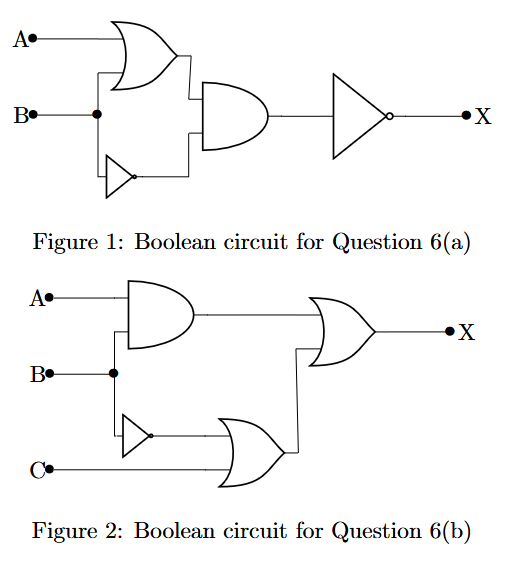
\includegraphics[width=0.7\textwidth]{HW3_figures.png}
\end{center}
Figure 1 Table \\ 
\[
\begin{array}{|c|c|c|c|c|c|c|}
	\hline
	A & B & A \lor B & \neg B & (A \lor B) \land \neg B & \neg((A \lor B) \land \neg B) & X \\
	\hline
	T & T & T & F & F & T & T \\
	T & F & T & T & T & F & F \\
	F & T & T & F & F & T & T \\
	F & F & F & T & F & T & T \\
	\hline
\end{array}
\]

Figure 2 Table \\ 
$
\begin{array}{|c|c|c|c|c|c|c|c|c|}
	\hline
	A & B & C & A \land B & \neg A & \neg B & \neg B \lor C & (A \land B) \lor (\neg B \lor C) & X \\
	\hline
	T & T & T & T & F & F & T & T & T \\
	T & T & F & T & F & F & F & T & T \\
	T & F & T & F & F & T & T & T & T \\
	T & F & F & F & F & T & T & T & T \\
	F & T & T & F & T & F & T & T & T \\
	F & T & F & F & T & F & F & F & F \\
	F & F & T & F & T & T & T & T & T \\
	F & F & F & F & T & T & T & T & T \\
	\hline
\end{array}
$
		 
		\item For each of the following tables construct:
		\begin{itemize}
			\item[(a)] A Boolean expression having the given table as its truth table and 
			\item[(b)] A circuit having the given table as its input/output table.
		\end{itemize}
		\[
		\begin{array}{|c|c|c|c|}
			\hline
			A & B & C & X \\
			\hline
			1 & 1 & 1 & 0 \\
			1 & 1 & 0 & 1 \\
			1 & 0 & 1 & 0 \\
			1 & 0 & 0 & 0 \\
			0 & 1 & 1 & 1 \\
			0 & 1 & 0 & 0 \\
			0 & 0 & 1 & 0 \\
			0 & 0 & 0 & 0 \\
			\hline
		\end{array}
		\]
		Looking at row 2 and 5 where the final result is 1: \\ 
		Row 2: $A \land B \land \neg C$ \\ 
		Row 5: $\neg A \land B \land C$ \\ 
		Boolean Expression : ( $A \land B \land \neg C$) $\lor$ ($\neg A \land B \land C$)
		
		\begin{figure}[!ht]
			\centering
			\resizebox{1\textwidth}{!}{%
				\begin{circuitikz}
					\tikzstyle{every node}=[font=\LARGE]
					\draw (6.5,17.75) to[short] (6.75,17.75);
					\draw (6.5,17.25) to[short] (6.75,17.25);
					\draw (6.75,17.75) node[ieeestd and port, anchor=in 1, scale=0.89](port){} (port.out) to[short] (8.5,17.5);
					\draw (6.75,18.75) node[ieeestd not port, anchor=in](port){} (port.out) to[short] (8.5,18.75);
					\draw (port.in) to[short] (6.5,18.75);
					\draw (6.5,16.5) to[short] (6.75,16.5);
					\draw (6.5,16) to[short] (6.75,16);
					\draw (6.75,16.5) node[ieeestd and port, anchor=in 1, scale=0.89](port){} (port.out) to[short] (8.5,16.25);
					\draw (8.5,18.75) to[short] (9.5,18.75);
					\draw (8.5,16.25) to[short] (9.5,16.25);
					\draw (10,17.75) to[short] (10.25,17.75);
					\draw (10,17.25) to[short] (10.25,17.25);
					\draw (10.25,17.75) node[ieeestd and port, anchor=in 1, scale=0.89](port){} (port.out) to[short] (12,17.5);
					\draw (10,17.75) to[short] (10,18.75);
					\draw (10,18.75) to[short] (9.5,18.75);
					\draw (10,17.25) to[short] (10,16.25);
					\draw (10,16.25) to[short] (9.5,16.25);
					\draw (10,15.75) to[short] (10.25,15.75);
					\draw (10,15.25) to[short] (10.25,15.25);
					\draw (10.25,15.75) node[ieeestd and port, anchor=in 1, scale=0.89](port){} (port.out) to[short] (12,15.5);
					\draw (10,15.25) to[short] (10,14.75);
					\draw (10,14.75) to[short] (8,14.75);
					\draw (8.5,17.5) to[short] (9.5,17.5);
					\draw (9.5,17.5) to[short] (9.5,15.75);
					\draw (9.5,15.75) to[short] (10,15.75);
					\draw (6.5,14.75) node[ieeestd not port, anchor=in](port){} (port.out) to[short] (8.25,14.75);
					\draw (port.in) to[short] (6.25,14.75);
					\draw (12.5,16.75) to[short] (13,16.75);
					\draw (12.5,16.25) to[short] (13,16.25);
					\draw (13,16.75) node[ieeestd or port, anchor=in 1, scale=0.89](port){} (port.out) to[short] (15,16.5);
					\draw (12.5,16.75) to[short] (12.5,17.5);
					\draw (12.5,17.5) to[short] (11.75,17.5);
					\draw (12.5,16.25) to[short] (12.5,15.5);
					\draw (12.5,15.5) to[short] (12,15.5);
					\node [font=\LARGE] at (15,16.5) {X};
					\node [font=\LARGE] at (5.5,19) {A};
					\node [font=\LARGE] at (5.5,15) {C};
					\node [font=\LARGE] at (5.5,19) {A};
					\node [font=\LARGE] at (5.5,19) {A};
					\node [font=\LARGE] at (5.5,19) {A};
					\node [font=\LARGE] at (5.5,19) {A};
					\node [font=\LARGE] at (5.5,19) {A};
					\node [font=\LARGE] at (5.5,19) {A};
					\draw (6.25,14.75) to[short] (5.75,14.75);
					\draw (6.5,16) to[short] (5.75,15.25);
					\draw (6.5,18.75) to[short] (5.75,18.75);
					\draw (6.5,17.75) to[short] (5.75,18.5);
					\draw (6.5,16.5) to[short] (6,17);
					\draw (6.5,17.25) to[short] (6,17.25);
					\node [font=\LARGE] at (5.5,17) {B};
				\end{circuitikz}
			}%
			
			\label{fig:my_label}
		\end{figure}

		\[
		\begin{array}{|c|c|c|c|}
			\hline
			A & B & C & X \\
			\hline
			1 & 1 & 1 & 0 \\
			1 & 1 & 0 & 1 \\
			1 & 0 & 1 & 0 \\
			1 & 0 & 0 & 0 \\
			0 & 1 & 1 & 1 \\
			0 & 1 & 0 & 1 \\
			0 & 0 & 1 & 0 \\
			0 & 0 & 0 & 0 \\
			\hline
		\end{array}
		\]
		Looking at row 2, 5 and 6 where the final result is 1: \\
		Row 2: $A \land B \neg C$ \\
		Row 5: $\neg A \land B \land C$ \\
		Row 6: $\neg A \land B \land \neg C$ \\
		Boolean Expression: $(A \land B \neg C)\lor (\neg A \land B \land C) \lor (\neg A \land B \land \neg C)$
		
		
		\begin{figure}[!ht]
			\centering
			\resizebox{1\textwidth}{!}{%
				\begin{circuitikz}
					\tikzstyle{every node}=[font=\LARGE]
					\draw (6.5,17.75) to[short] (6.75,17.75);
					\draw (6.5,17.25) to[short] (6.75,17.25);
					\draw (6.75,17.75) node[ieeestd and port, anchor=in 1, scale=0.89](port){} (port.out) to[short] (8.5,17.5);
					\draw (6.75,18.75) node[ieeestd not port, anchor=in](port){} (port.out) to[short] (8.5,18.75);
					\draw (port.in) to[short] (6.5,18.75);
					\draw (6.5,16.5) to[short] (6.75,16.5);
					\draw (6.5,16) to[short] (6.75,16);
					\draw (6.75,16.5) node[ieeestd and port, anchor=in 1, scale=0.89](port){} (port.out) to[short] (8.5,16.25);
					\draw (8.5,18.75) to[short] (9.5,18.75);
					\draw (8.5,16.25) to[short] (9.5,16.25);
					\draw (10,17.75) to[short] (10.25,17.75);
					\draw (10,17.25) to[short] (10.25,17.25);
					\draw (10.25,17.75) node[ieeestd and port, anchor=in 1, scale=0.89](port){} (port.out) to[short] (12,17.5);
					\draw (10,17.75) to[short] (10,18.75);
					\draw (10,18.75) to[short] (9.5,18.75);
					\draw (10,17.25) to[short] (10,16.25);
					\draw (10,16.25) to[short] (9.5,16.25);
					\draw (10,15.75) to[short] (10.25,15.75);
					\draw (10,15.25) to[short] (10.25,15.25);
					\draw (10.25,15.75) node[ieeestd and port, anchor=in 1, scale=0.89](port){} (port.out) to[short] (12,15.5);
					\draw (10,15.25) to[short] (10,14.75);
					\draw (10,14.75) to[short] (8,14.75);
					\draw (8.5,17.5) to[short] (9.5,17.5);
					\draw (9.5,17.5) to[short] (9.5,15.75);
					\draw (9.5,15.75) to[short] (10,15.75);
					\draw (6.5,14.75) node[ieeestd not port, anchor=in](port){} (port.out) to[short] (8.25,14.75);
					\draw (port.in) to[short] (6.25,14.75);
					\draw (12.5,16.75) to[short] (13,16.75);
					\draw (12.5,16.25) to[short] (13,16.25);
					\draw (13,16.75) node[ieeestd or port, anchor=in 1, scale=0.89](port){} (port.out) to[short] (15,16.5);
					\draw (12.5,16.75) to[short] (12.5,17.5);
					\draw (12.5,17.5) to[short] (11.75,17.5);
					\draw (12.5,16.25) to[short] (12.5,15.5);
					\draw (12.5,15.5) to[short] (12,15.5);
					\node [font=\LARGE] at (18.75,18) {X};
					\node [font=\LARGE] at (5.5,19) {A};
					\node [font=\LARGE] at (5.5,15) {C};
					\node [font=\LARGE] at (5.5,19) {A};
					\node [font=\LARGE] at (5.5,19) {A};
					\node [font=\LARGE] at (5.5,19) {A};
					\node [font=\LARGE] at (5.5,19) {A};
					\node [font=\LARGE] at (5.5,19) {A};
					\node [font=\LARGE] at (5.5,19) {A};
					\draw (6.25,14.75) to[short] (5.75,14.75);
					\draw (6.5,16) to[short] (5.75,15.25);
					\draw (6.5,18.75) to[short] (5.75,18.75);
					\draw (6.5,17.75) to[short] (5.75,18.5);
					\draw (6.5,16.5) to[short] (6,17);
					\draw (6.5,17.25) to[short] (6,17.25);
					\node [font=\LARGE] at (5.5,17) {B};
					\draw (10,18.75) to[short] (12.5,18.75);
					\draw (10,14.75) to[short] (12,14.75);
					\draw (12,14.75) to[short] (12,18.25);
					\draw (12,18.25) to[short] (12.5,18.25);
					\draw (12.5,18.75) to[short] (12.75,18.75);
					\draw (12.5,18.25) to[short] (12.75,18.25);
					\draw (12.75,18.75) node[ieeestd and port, anchor=in 1, scale=0.89](port){} (port.out) to[short] (14.5,18.5);
					
					\draw (14.5,18) to[short] (14.5,17.25);
					\draw (14.5,17.25) to[short] (11.75,17.25);
					\draw (11.75,17.25) to[short] (11.75,16.75);
					\draw (11.75,16.75) to[short] (8.25,16.75);
					\draw (8.25,16.75) to[short] (6.25,16.75);
					\draw (14.5,18.5) to[short] (14.75,18.5);
					\draw (14.5,18) to[short] (14.75,18);
					\draw (14.75,18.5) node[ieeestd and port, anchor=in 1, scale=0.89](port){} (port.out) to[short] (16.5,18.25);
					\draw (16.5,18.25) to[short] (16.75,18.25);
					\draw (16.5,17.75) to[short] (16.75,17.75);
					\draw (16.75,18.25) node[ieeestd or port, anchor=in 1, scale=0.89](port){} (port.out) to[short] (18.5,18);
					\draw (16.5,17.75) to[short] (16.5,16.5);
					\draw (15,16.5) to[short] (16.5,16.5);
				\end{circuitikz}
			}%
			
		\end{figure}
		
		\item Let $Q(x, y)$ be the predicate "If $x < y$ then $x^2 < y^2$" with domain for both $x$ and $y$ being the set $\mathbb{R}$ of real numbers.
		\begin{itemize}
			\item[(a)] Explain why $Q(x, y)$ is false if $x = -2$ and $y = 1$.
			\item[$\vdots$] -2 < 1, but 4 $\not<$ 1
			\item[(b)] Give values different from those in part (a) for which $Q(x, y)$ is false.
			\item[$\vdots$] -5 < 3, 25 $\not<$ 6 
			\item[(c)] Explain why $Q(x, y)$ is true if $x = 3$ and $y = 8$.
			\item[$\vdots$] 3 < 8, 9 < 64. It is true because 9 is less than 64
			\item[(d)] Try to add a universal quantifier before the predicate so that the predicate is always true.
			\item[$\vdots$] We can modify the predicate and limit the domain to all non-negative numbers : \\
			$\forall x,y \in \mathbb{R}^+, (x,y \rightarrow x^2,y^2)$ \\ 
			Otherwise, if would be impossible to work with the domain of real numbers since it includes negative values and we have proven that -2 < 1 but the squares of both: 4 $\not<$ 1 is false.
			
		\end{itemize}
		
		
		\item Let $D$ be the set of all students at FIU, and let $M(s)$ be "s is a math major", $C(s)$ be "s is a computer science student", and $E(s)$ be "s is an engineering student". Express each of the following statements using quantifiers, variables, and the predicates $M(s)$, $C(s)$, and $E(s)$.
		\begin{itemize}
			\item[(a)] There is an engineering student who is a math major.
			\item[$\vdots$] \(\exists s \in D \, (E(s) \land M(s))\)
			\item[(b)] Every computer science student is an engineering student.
			\item[$\vdots$] \(\forall s \in D \, (C(s) \Rightarrow E(s))\)
			
			\item[(c)] No computer science students are engineering students.
			\item[$\vdots$] \(\forall s \in D \, (C(s) \Rightarrow \neg E(s))\)
			
			\item[(d)] Some computer science students are also math majors.
			\item[$\vdots$] \(\exists s \in D \, (C(s) \land M(s))\)
			
			\item[(e)] Some computer science students are engineering students and some are not.
			\item[$\vdots$] \(\exists s_1 \in D \, (C(s_1) \land E(s_1)) \land \exists s_2 \in D \, (C(s_2) \land \neg E(s_2))\)
			
		\end{itemize}
		
		\item For each of the following statements:
		\begin{itemize}
			\item[(a)] Rewrite the statement formally using quantifiers and variables, and
			\item[(b)] Write a negation for the statement.
		\end{itemize}
		\begin{itemize}
			\item[(a)] Everybody loves somebody.
			\item[--] for every person x, there exists y such that x loves y \\
					$\forall x \exists y$  $L(x,y)$ \\
					Negation: $\exists x \forall y$ $\neg L(x,y)$ \\ 
					
			\item[(b)] Somebody loves everybody.
			\item[--] there exists x, for every person y, such that x loves y \\
					$\exists x \forall y$ $L(x,y)$ \\ 
					Negation: $\forall x \exists y$ $ \neg L(x,y)$
		\end{itemize}
	\end{enumerate}
	
\end{document}
